\chapter{Experiments}
In this chapter, the presented algorithmic approaches are experimentally evaluated on sets of procedurally generated instances with different features, including instances of both the problem with and without fixed seed tile. Furthermore, we investigate the impact of several parameters, such as the number of tiles, the size of the board, the placement of obstacles, etc., on the difficulty of the problem. The main focus of the analysis is on the comparison of runtimes and the quality (length) of the found solutions. Additionally, the memory requirements of our implementations and the effectiveness of the proposed solution shortening method are briefly evaluated.

\section{Method for Instance Creation}

\begin{figure}
\centering
\begin{subfigure}[b]{0.45\textwidth}
\centering
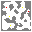
\includegraphics[width=\textwidth]{figures/example_boards/cave_example.pdf}
\caption{Example cave board instance}
\label{fig:cave}
\end{subfigure}
\hfill
\begin{subfigure}[b]{0.45\textwidth}
\centering
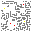
\includegraphics[width=\textwidth]{figures//example_boards/maze_example.pdf}
\caption{Example maze board instance}
\label{fig:maze}
\end{subfigure}
\caption[Example instances for the two different board types]{Example instances for the two different board types. The grey squares represent blocked positions and the colored squares are tiles. The red-striped area marks the target shape. The border is implicitly considered as blocked.}
\label{fig:instance_example}
\end{figure}

To create a sufficient number of instances with a range of different features for experimentation, we implemented a Python function, that procedurally generates such instances based on six input parameters.
\begin{enumerate}
\setlength\itemsep{-0.3em}
\item \textbf{Board type:} This parameter decides which randomized algorithm is used to determine the blocked positions on the board. Two different board types were used for the experiments. The first type is called \emph{maze} and boards of this type are created in a two-step process. Firstly, starting on a board filled with blocked positions, a randomized recursive backtracking algorithm creates a tree of open spaces. Secondly, a number of rectangular open regions proportional to the size of the board is added uniformly at random. The second type is called \emph{cave}. Boards of this type are created using cellular automata, with the following rules: A dead cell becomes alive in the next generation if it has 5 or more living neighbors. A living cell becomes dead in the next generation if it has less than 4 living neighbors. After applying two generations of these rules to a grid where each cell starts alive with a probability of $0.45$, the positions of the living cells correspond to the blocked positions on the cave board. Additionally, to ensure connectedness, the largest connected component of open spaces is determined and all other open spaces are filled. The idea is to create boards with different properties in order to evaluate the influence of obstacle placement on the motion planning algorithms. Maze boards contain open areas, that are connected through narrow corridors; whereas cave boards contain fewer narrow sections.
\item \textbf{Target shape size:}
The number of tiles that are required to assemble the target shape.
\item \textbf{Board size:}
For the experiments, only square-shaped boards were used. The board size determines the edge length of the board.
\item \textbf{Number of extra tiles:}
The number of tiles added to the initial configuration which are not needed to create the target shape. The total number of tiles is the sum of the target shape size and the number of extra tiles.
\item \textbf{Number of glues:}
The number of different glues. The glues on the edges of each tile are selected uniformly at random from the set of available glues. To make it more likely for instances to have a solution, a subset of the tiles is arranged into the target shape and a set of rules is added such that they bond. Finally, additional rules are selected at random, until at least half of all possible combinations of glues stick together.
\item \textbf{Problem type:}
The problem type determines whether a fixed seed tile exists or not. If a fixed seed tile exists, tiles can only bond, if the resulting polyomino contains the fixed tile.
\end{enumerate}

To determine the initial tile positions, tiles are successively placed on legal positions uniformly at random. A position is considered legal, if it is open, does not contain a tile, and is not adjacent to a position containing a tile. The last condition ensures that the initial configuration only contains $1 \times 1$ polyominoes. If a fixed seed tile is required, it is placed first on a suitable position within the target shape. On all generated boards, the open positions form a connected region. Although some measures were taken to increase the probability that the created instances are solvable, instances are not guaranteed to have a solution.

\section{Experimental Setup}
This section explains the methods and tools we used for the experiments and provides an overview of the evaluated algorithmic approaches.

\subsection{Simulation Environment}
For the experiments, all discussed motion planning algorithms were implemented in a self-developed simulator, which is based on TumbleTiles \footnote{TumbleTiles on Github: \url{https://github.com/asarg/TumbleTiles}}. The original TumbleTiles software was upgraded from Python 2 to Python 3 and heavily modified. It is capable of simulating step transformations on configurations with and without fixed seed tile. Furthermore, we implemented support for custom glue functions. Additionally, the software features a GUI that allows the user to view and edit a configuration, animate step sequences, and execute the various motion planning algorithms. \par
The experiments were conducted on multiple computers, each with the same specifications (\textbf{Intel(R) Core(TM) i7-6700K CPU @ 4x4.00GHz, 64GB RAM}) running Ubuntu 20.04 LTS. Multiple motion planning algorithms were evaluated at the same time using different CPU cores.

\subsection{Evaluated Approaches}
This subsection provides an overview of the $10$ evaluated motion planning algorithms and the abbreviations that will be used to refer to them in the following. Furthermore, details about the used parameters are listed if required.
\begin{enumerate}
\setlength\itemsep{0.2em}
\item Breadth-first-search (BFS)
\item Greatest Distance heuristic (GD)
\item Average Distance heuristic (AD)
\item Greedy Greatest Distance heuristic (GGD)
\item Greedy Average Distance heuristic (GAD)
\item Weighted Sum of Distances heuristic (WSD): $e =2$.
\item Minimum Moves to Polyomino heuristic (MMP)
\item Minimum Moves to Polyomino or Target area heuristic (MMPT): $d_t = 4$.
\item Distance to Fixed Position heuristic (DFP)
\item Rapidly-exploring Random Tree (RRT): The Hausdorf-distance based on the shortest path length is used as the cost-to-go function. Each expansion step consists of $40$ iterations of a greedy best-first search. The bias towards the goal is $5$\%. Below a threshold distance of $7$ or less to the goal, a best-first search limited to $500$ iterations attempts to find a solution.
\end{enumerate}

For each solver, all applicable pruning methods discussed in Chapter 3 were used.
Additionally, in combination with the all-tiles-at-the-same-time heuristic approaches (GD, AD, GGD, GAD, WSD) the alternative stop condition from Section 3.2.1 was used, if the configuration contained no extra tiles.

\subsection{Experimental Procedure}
The motion planning algorithms were evaluated on two sets of instances, which were created in advance and contain the same instances for every experiment.

\paragraph{\texttt{InstanceSet1}} consists of relatively easy to solve instances, that allow a comparison of all solvers, including the breadth-first search solver and other (near-)optimal solvers. It contains 5 procedurally generated instances for each possible combination of parameters from the following table.
\begin{center}
\begin{tabular}{ |l|r| }
\hline
Board type & cave, maze \\
\hline
Target shape size & $3 , 4, 5 , 6$ \\
\hline
Board size & $20 , 30, 40$ \\
\hline
Extra tiles & $0, 1, 3$ \\
\hline
Number of glues & $1 , 2, 3$ \\
\hline
Problem type & $\text{seed tile}, \text{no seed tile}$ \\
\hline
% \caption[Possible parameters for \texttt{InstanceSet1}]{The values of parameters used for the creation of the instances in \texttt{InstanceSet1}}

\end{tabular}
\end{center}

\paragraph{\texttt{InstanceSet2}} consists of instances with a wider range of difficulties. It contains 5 procedurally generated instances or each possible combination of parameters from the following table.
\begin{center}
\begin{tabular}{ |l|r| }
\hline
Board type & cave, maze \\
\hline
Target shape size & $5, 10, 13, 15$ \\
\hline
Board size & $40, 80, 120$ \\
\hline
Extra tiles & $0, 3, 5$ \\
\hline
Number of glues & $1, 3, 5$ \\
\hline
Problem type & $\text{seed tile}, \text{no seed tile}$ \\
\hline
\end{tabular}
% \caption[Possible parameters for \texttt{InstanceSet2}]{The values of parameters used for the creation of the instances in \texttt{InstanceSet2}}
\end{center}

\par

Both sets contain a total of $2160$ instances each. The instances from \texttt{InstanceSet1} were attempted to solve with all $10$ evaluated algorithms, whereas only selected solvers (GAD, WSD, MMPT, DFP) were used for \text{InstanceSet2}. DFP was only used on suitable instances, i.e. instances with a fixed seed tile. \par
All experiments were conducted with a timeout of 600 seconds per instance, after which the motion planning algorithm was stopped if it did not find a solution or proved that no solution exists.\par
Along with the problem instance, the solution sequence (if solved), the runtime, and the peak memory usage were recorded. Additionally, the number of nodes in the search tree, or in the case of one-tile-at-a-time algorithms the sum of nodes in all search trees, was recorded.

\begin{figure}[h]
\centering
\includegraphics[width=0.8\textwidth]{figures/example_boards/exampleboards_annotated.pdf}
\caption [Runtime comparison by problem type for GAD] {Six randomly generated instances of different board sizes from \texttt{InstanceSet1}, three cave boards on the left and three maze boards on the right. The yellow squares are tiles and the red-stripped polyominoes are the target shapes. Glues are not shown.}
\label{fig:example_boards}
\end{figure}



\section{Results}

In this section, our algorithmic approaches are evaluated using the experiment results from both sets of instances.

\subsection{Evaluation of \texttt{InstanceSet1}}

The experiment results from \texttt{InstanceSet1} are used to measure the impact of various parameters on the performance of different motion planning algorithms. The relatively small size of the instances allows every solver including the breadth-first search approach and other near-optimal motion planners to solve a large fraction of instances within the timeout of 10 minutes. This provides a baseline for the performance of the other solvers. Additionally, this data is used to evaluate the impact of several configuration parameters on the efficiency of the different motion planning algorithms and to compare the memory requirements of the different approaches as well as the effectiveness of our solution shortening method.

\subsubsection {Performance of breadth-first search}

Figures \ref{fig:bfs_performance1}, \ref{fig:bfs_performance2} show the runtime distribution and the fraction of instances that were successfully solved within the timeout
for instances with a small number of tiles. Note that the performance decreases sharply with an
increased number of tiles. At 3 tiles, more than $70\%$ were successfully solved or shown to have no solution, whereas at 5 tiles less than $10\%$ of instances were finished before the timeout. Only one instance with 9 tiles was successfully solved. The size of the board also had a significant impact on the performance of the solver. Furthermore, a majority of the solved instances were solved long before the timeout. \\
The length of the solutions found by the BFS solver seems to decrease when the number of tiles on the board increases, as shown in Figure \ref{fig:bfs_performance3}. There are two possible reasons for this. Firstly, an increased density of tiles on the board allows shorter solution sequences for target shapes of the same size. Secondly, for a larger number of tiles, the solver only found a solution before the timeout if a relatively short solution existed. \\
In contrast, the solution length significantly increases with increasing board size.
\newpage

\begin{figure}[H]
\centering
\begin{subfigure}[b]{\textwidth}
\centering
\includegraphics[width=\textwidth]{figures/plots/heuristic_solvers_i1/bfs_time_over_tiles.pdf}
\caption{Runtime distributions by number of tiles as box plot. Only successful solutions are shown.}
\label{fig:bfs_time_over_tiles}
\end{subfigure}
\begin{subfigure}[b]{\textwidth}
\centering
\includegraphics[width=\textwidth]{figures/plots/heuristic_solvers_i1/bfs_time_over_board_size.pdf}
\caption{Runtime distributions by board size as box plot. Only successful solutions are shown.}
\label{fig:bfs_fraction_solved_over_board_size}
\end{subfigure}
\caption[Runtime of the BFS motion planner on \texttt{InstanceSet1}] {Runtime of the Breadth-first-search (BFS) motion planner on \texttt{InstanceSet1} by number of tiles and board size. The boxes show upper and lower quartile, the line the median, the whiskers extend to the most extreme value that is within a proportion of 1.5 of the interquartile range. The white dot indicates the arithmetic mean and the other dots outliers.
All experiments were conducted with a 600 seconds timeout per instance, as shown by the dotted red line.}
\label{fig:bfs_performance1}
\end{figure}
\begin{figure}[H]
\begin{subfigure}[b]{\textwidth}
\centering
\includegraphics[width=\textwidth]{figures/plots/heuristic_solvers_i1/bfs_fraction_solved_over_tiles.pdf}
\caption {Fraction of solved instances by number of tiles.}
\label{fig:bfs_fraction_solved_over_tiles}
\end{subfigure}
\begin{subfigure}[b]{\textwidth}
\centering
\includegraphics[width=\textwidth]{figures/plots/heuristic_solvers_i1/bfs_fraction_solved_over_board_size.pdf}
\caption{Fraction of solved instances by board size.}
\label{fig:bfs_fraction_solved_over_board_size}
\end{subfigure}
\caption [Fraction of \texttt{InstanceSet1} solved by the BFS motion planner] {Fraction of instances from \texttt{InstanceSet1} that were solved by the BFS motion planner or for which the solver determined that no solution exists by number of tiles and board size.}
\label{fig:bfs_performance2}
\end{figure}
\begin{figure}[H]
\begin{subfigure}[b]{\textwidth}
\centering
\includegraphics[width=\textwidth]{figures/plots/heuristic_solvers_i1/bfs_solution_length_over_tiles.pdf}
\caption{Distribution of solution length by number of tiles as box plot.}
\label{fig:bfs_solution_length_over_tiles}
\end{subfigure}
\begin{subfigure}[b]{\textwidth}
\centering
\includegraphics[width=\textwidth]{figures/plots/heuristic_solvers_i1/bfs_solution_length_over_board_size.pdf}
\caption{Distribution of solution length by board size as box plot.}
\label{fig:bfs_solution_length_over_board_size}
\end{subfigure}
\caption[Solution lengths for BFS motion planner on \texttt{InstanceSet1}]{Solution length for the BFS motion planner on \texttt{InstanceSet1} by tiles and board size. Only instances for which a solution was found are taken into account.}
\label{fig:bfs_performance3}
\end{figure}


\subsubsection {Comparision of the all-tiles-at-the-same-time search-based motion planning algorithms}


In this subsection, the performance of the BFS solver and the search-based motion planning algorithms GD, AD, GGD, GAD, and WSD are compared. All of these algorithms are best-first searches that try to minimize a function of the distance of multiple tiles to the target shape.\\
As expected, all heuristic searches show a better performance in terms of runtime and success rate than breadth-first search (see Figures \ref{fig:hs_i1_performance1}, \ref{fig:hs_i1_performance2}). The A* searches with consistent heuristic GD and AD take clearly longer to find a solution and have a lower success rate, especially on instances with greater numbers of tiles, than the greedy best-first search approaches. Interestingly, the GD algorithm seems to perform better than the AD algorithm, whereas the greedy algorithms GGD, GAD, and WSD all show a similar performance. All solvers show a clear decrease in success rate with an increasing number of tiles, whereas for the investigated board sizes GAD and WSD show low sensitivity to a change in board size. Overall, the number of tiles seems to have the greatest impact on the performance. \\
The near-optimal motion planning algorithms expectedly produce solutions of roughly the same length as shown in Figure \ref{fig:hs_i1_performance3}. On the other hand, the solution length for the greedy algorithms was much longer on average and they show clear differences in the quality of the found solutions. The solutions found by GAD and WSD are usually shorter than solutions found by GGD. Again, the size of the board seems to have a greater impact than the number of tiles on the length of the found solution.
However, the solution length of GGD seems to be more sensitive to the number of tiles than other approaches. Since the heuristic value of a configuration in GGD only represents the distance of a single tile to the target shape, the distance of a growing number of tiles to the target shape is ignored, when a large number of tiles is present, which may explain this trend.\\
On instances where both AD and GAD found a solution, the solution of the greedy approach was longer than the near-optimal solution of the A* approach by a factor of $2.96$ on average. However, this factor decreases with an increase in board size as the following table indicates. \\

\begin{center}
\begin{tabular}{ |l|r| }
\hline
Board size & $\text{GAD} / \text{AD}$ solution, mean ratio\\
\hline
$20 \times 20$ & $3.24 \pm 3.78$ \\
\hline
$30 \times 30$ & $2.64 \pm 2.31$ \\
\hline
$40 \times 40$ & $2.49 \pm 2.52$ \\
\hline
\end{tabular}
\captionof{table}{Mean ratio of the length of a solution found by GAD and the solution to the same instance found by AD to 3 significant figures $\pm \text{SD}$ for different board sizes.}
\end{center}

\begin{figure}[H]
\centering
\begin{subfigure}[b]{\textwidth}
\centering
\includegraphics[width=\textwidth]{figures/plots/heuristic_solvers_i1/hs_i1_time_over_tiles.pdf}
\caption{Runtime distributions by number of tiles as box plot. Only successful solutions are shown.}
\label{fig:hs_i1_time_over_tiles}
\end{subfigure}
\begin{subfigure}[b]{\textwidth}
\centering
\includegraphics[width=\textwidth]{figures/plots/heuristic_solvers_i1/hs_i1_time_over_board_size.pdf}
\caption{Runtime distributions by board size as box plot. Only successful solutions are shown.}
\label{fig:hs_i1_time_over_board_size}
\end{subfigure}
\caption[Runtime of the search-based heuristic planners on \texttt{InstanceSet1}]{Comparison of the runtime of search-based heuristic motion planning algorithms on \texttt{InstanceSet1} by number of tiles and board size.}
\label{fig:hs_i1_performance1}
\end{figure}
\begin{figure}[H]
\begin{subfigure}[b]{\textwidth}
\centering
\includegraphics[width=\textwidth]{figures/plots/heuristic_solvers_i1/hs_i1_fraction_solved_over_tiles.pdf}
\caption{Fraction of solved instances by number of tiles.}
\label{fig:hs_i1_fraction_solved_over_tiles}
\end{subfigure}
\begin{subfigure}[b]{\textwidth}
\centering
\includegraphics[width=\textwidth]{figures/plots/heuristic_solvers_i1/hs_i1_fraction_solved_over_board_size.pdf}
\caption{Fraction of solved instances by board size.}
\label{fig:hs_i1_fraction_solved_over_board_size}
\end{subfigure}
\caption [Fraction of \texttt{InstanceSet1} solved by the search-based planners] {Fraction of instances from \texttt{InstanceSet1} that were solved by search-based heuristic motion planning algorithms by number of tiles and board size.}
\label{fig:hs_i1_performance2}
\end{figure}
\begin{figure}[H]
\begin{subfigure}[b]{\textwidth}
\centering
\includegraphics[width=\textwidth]{figures/plots/heuristic_solvers_i1/hs_i1_solution_length_over_tiles.pdf}
\caption{Distribution of solution length by number of tiles as box plot.}
\label{fig:hs_i1_solution_length_over_tiles}
\end{subfigure}
\begin{subfigure}[b]{\textwidth}
\centering
\includegraphics[width=\textwidth]{figures/plots/heuristic_solvers_i1/hs_i1_solution_length_over_board_size.pdf}
\caption{Distribution of solution length by board size as box plot.}
\label{fig:hs_i1_solution_length_over_board_size}
\end{subfigure}
\caption[Solution lengths for search-based heuristic planners on \texttt{InstanceSet1}]{Comparison of the solution length of different search-based heuristic motion planning algorithms on \texttt{InstanceSet1} by tiles and board size. Only instances for which a solution was found are taken into account. Outliers are omitted for better readability.}
\label{fig:hs_i1_performance3}
\end{figure}

\newpage

\subsubsection{Effects of the alternative stop condition}

The alternative stop condition that was used only in the absence of extra tiles causes the near-optimal solvers to find solutions that are within the largest possible distance on the board of the optimal solution. In exchange, sometimes a solution can be found after fewer expanded nodes. Figure \ref{fig:moves_to_target} shows the distributions of steps required to move the assembled final polyomino to the target shape. Note that the BFS algorithm on average assembles the polyomino much further away from the target shape position. The heuristics, which are based on the distance of tiles to the target shape, cause configurations with tiles closer to the target shape to be expanded first. Therefore, the target polyomino is more likely to be assembled close to its target position. In contrast, for the BFS solver, it does not matter where on the board the target polyomino is assembled as long as the target shape position is reachable. This suggests, that for the heuristic-based solvers the impact of the alternative stop condition on the solution length was negligible.

\begin{figure}[htpb]
\centering
\includegraphics[width=\textwidth]{figures/plots/heuristic_solvers_i1/hs_i1_moves_to_target_over_board_size.pdf}
\caption[Number of steps after assembly of the final polyomino]{Boxplot comparison of the number of steps needed to move the assembled target polyomino to the target position for different heuristics, grouped by the size of the board. Only the instances where the alternative stop condition was used are shown.}
\label{fig:moves_to_target}
\end{figure}

\vfill
\newpage

\subsubsection{Performance of the remaining motion planning algorithms}

In this subsection, the performance of the remaining approaches, consisting of the one-tile-at-a-time motion planning algorithms (MMP, MMPT, DFP), as well as RRT, will be investigated. For comparison, GAD is included in the plots.
As shown in Figures \ref{fig:i1_performance1}, \ref{fig:i1_performance2} all one-tile-at-a-time algorithms display a better success rate than GAD on instances with a number of tiles greater than 5. The runtime on instances with many tiles is clearly better too. However, the runtime of MMP appears to be particularly sensitive to an increase in board size.
MMPT does not have this downside and shows superior performance to MMP.
In general, the performance of the one-tile-at-a-time approach seems to degrade much slower than the performance of other approaches when the number of tiles is increased.
\\
The DFP motion planner can only be evaluated on instances of the Fixed Seed Tile Polyomino Assembly Problem. It has a high success rate of around $90\%$ on these instances regardless of the number of tiles and the size of the board. Furthermore, a large majority of instances that are solved by DFP are solved in less than 1 second. \\
RRT displays a similar behavior as GAD but its runtime is more sensitive to increased board size. \\
Regarding the solution lengths, shown in Figure \ref{fig:i1_performance3}, the one-tile-at-a-time algorithms usually produce shorter solutions than other approaches. The length of solutions found by RRT are on average shorter and exhibit lower variance than those found by GAD.
None of the solvers demonstrates a large effect of the number of tiles on the solution length. In contrast, an increased board size correlates with an increased solution length for all solvers.


\begin{figure}[htpb]
\centering
\begin{subfigure}[b]{\textwidth}
\centering
\includegraphics[width=\textwidth]{figures/plots/heuristic_solvers_i1/i1_time_over_tiles.pdf}
\caption{Runtime distributions by number of tiles as box plot. Only successful solutions are shown.}
\label{fig:hs_i1_time_over_tiles}
\end{subfigure}
\begin{subfigure}[b]{\textwidth}
\centering
\includegraphics[width=\textwidth]{figures/plots/heuristic_solvers_i1/i1_time_over_board_size.pdf}
\caption{Runtime distributions by board size as box plot. Only successful solutions are shown.}
\label{fig:hs_i1_time_over_board_size}
\end{subfigure}
\caption[Runtime of several planners on \texttt{InstanceSet1}]{Comparison of the runtime of several motion planning algoritms on \texttt{InstanceSet1} by number of tiles and board size. Outliers are omitted.}
\label{fig:i1_performance1}
\end{figure}
\begin{figure}[htpb]
\begin{subfigure}[b]{\textwidth}
\centering
\includegraphics[width=\textwidth]{figures/plots/heuristic_solvers_i1/i1_fraction_solved_over_tiles.pdf}
\caption{Fraction of solved instances by number of tiles.}
\label{fig:i1_fraction_solved_over_tiles}
\end{subfigure}
\begin{subfigure}[b]{\textwidth}
\centering
\includegraphics[width=\textwidth]{figures/plots/heuristic_solvers_i1/i1_fraction_solved_over_board_size.pdf}
\caption{Fraction of solved instances by board size.}
\label{fig:i1_fraction_solved_over_board_size}
\end{subfigure}
\caption [Fraction of \texttt{InstanceSet1} solved by several planners] {Fraction of instances from \texttt{InstanceSet1} that were solved by different motion planning algorithms by number of tiles and board size.}
\label{fig:i1_performance2}
\end{figure}
\begin{figure}[htpb]
\begin{subfigure}[b]{\textwidth}
\centering
\includegraphics[width=\textwidth]{figures/plots/heuristic_solvers_i1/i1_solution_length_over_tiles.pdf}
\caption{Distribution of solution length by number of tiles as box plot.}
\label{fig:i1_solution_length_over_tiles}
\end{subfigure}
\begin{subfigure}[b]{\textwidth}
\centering
\includegraphics[width=\textwidth]{figures/plots/heuristic_solvers_i1/i1_solution_length_over_board_size.pdf}
\caption{Distribution of solution length by board size as box plot.}
\label{fig:i1_solution_length_over_board_size}
\end{subfigure}
\caption[Solution lengths for several planners on \texttt{InstanceSet1}]{Comparison of the solution length of different motion planning algorithms on \texttt{InstanceSet1} by tiles and board size. Only instances for which a solution was found are taken into account.}
\label{fig:i1_performance3}
\end{figure}

\vfill
\newpage

\subsubsection{Comparison of the difficulty of the two problem types}

\texttt{InstanceSet1} contains instances of both the Polyomino Assembly Problem and the Fixed Seed Tile Polyomino Assembly Problem.
We compare the performance of three fundamentally different motion planning approaches for both problems in order to evaluate which problem is harder to solve in practice.
Figures \ref{fig:gad_fixed}, \ref{fig:mmpt_fixed}, \ref{fig:rrt_fixed} show the runtime performance of GAD, MMPT and RRT respectively. All three solvers demonstrate decisively better performance for the problem with a fixed seed tile. For less than 10 tiles, the time needed to solve an instance of the Fixed Seed Tile Polyomino Assembly Problem does not significantly increase when the number of tiles is increased. This is in stark contrast to instances of the Polyomino Assembly Problem where the runtime increases sharply.
Moreover, DFP provides a very efficient and reliable way to solve instances with fixed seed tile.


\begin{figure}[htpb]
\centering
\includegraphics[width=\textwidth]{figures/plots/heuristic_solvers_i1/gad_i1_fixed_time_over_tiles.pdf}
\caption [Runtime comparison by problem type for GAD] {Comparison of the runtime of the Polyomino Assembly Problem with and without fixed seed tile for the GAD solver by number of tiles.}
\label{fig:gad_fixed}
\end{figure}


\begin{figure}[htpb]
\centering
\includegraphics[width=\textwidth]{figures/plots/heuristic_solvers_i1/mmpt_i1_fixed_time_over_tiles.pdf}
\caption[Runtime comparison by problem type for MMPT]{Comparison of the runtime of the Polyomino Assembly Problem with and without fixed seed tile for the MMPT solver by number of tiles.}
\label{fig:mmpt_fixed}
\end{figure}

\begin{figure}[htpb]
\centering
\includegraphics[width=\textwidth]{figures/plots/heuristic_solvers_i1/rrt_i1_fixed_time_over_tiles.pdf}
\caption [Runtime comparison by problem type for RRT] {Comparison of the runtime of the Polyomino Assembly Problem with and without fixed seed tile for the RRT solver by number of tiles.}
\label{fig:rrt_fixed}
\end{figure}

\vfill

\subsubsection{Effect of the board type on the problem difficulty}

To investigate the effect of the obstacle placement, we compare the performance of motion planning algorithms on maze and cave boards (see Figures \ref{fig:i1_gad_maze_cave}, \ref{fig:i1_mmpt_maze_cave}, \ref{fig:i1_rrt_maze_cave}). GAD and RRT both display a similar success rate for both maze and cave boards, whereas MMPT solved slightly more cave boards than maze boards successfully. However, MMPT needed significantly more time for successful solves of cave boards compared to maze boards. This could indicate that, due to the different topography, undesired subassemblies are created more frequently on cave boards than on maze boards, which would cause the MMPT solver to spend more time trying to avoid the creation of subassemblies. Since GAD and RRT allow the creation of multiple subassemblies, they are less affected by this issue. \\
Across all solvers, the solution length on maze boards was higher than on cave boards of the same size, as shown in Figure \ref{fig:maze_vs_cave_solution_length}.
The reason for this could be the greater average pairwise distance between open spaces on maze boards (see Figure \ref{fig:maze_vs_cave_average_distance}).

\begin{figure}[htpb]
\begin{subfigure}[b]{\textwidth}
\centering
\includegraphics[width=\textwidth]{figures/plots/heuristic_solvers_i1/gad_i1_maze_vs_cave_time.pdf}
\caption{Runtime distributions by number of tiles as box plot. Only successful solutions are shown.}
\label{fig:i1_gad_maze_cave_time}
\end{subfigure}
\begin{subfigure}[b]{\textwidth}
\centering
\includegraphics[width=\textwidth]{figures/plots/heuristic_solvers_i1/gad_i1_maze_vs_cave_fraction_solved.pdf}
\caption{Fraction of solved instances by number of tiles.}
\label{fig:i1_gad_maze_cave_fraction_solved}
\end{subfigure}
\caption[Runtime and success rate of GAD on maze and cave boards]{Comparison of the runtimes and success rates of the GAD motion planner on maze and cave boards by number of tiles.}
\label{fig:i1_gad_maze_cave}
\end{figure}

\begin{figure}[htpb]
\begin{subfigure}[b]{\textwidth}
\centering
\includegraphics[width=\textwidth]{figures/plots/heuristic_solvers_i1/mmpt_i1_maze_vs_cave_time.pdf}
\caption{Runtime distributions by number of tiles as box plot.}
\label{fig:i1_mmpt_maze_cave_time}
\end{subfigure}
\begin{subfigure}[b]{\textwidth}
\centering
\includegraphics[width=\textwidth]{figures/plots/heuristic_solvers_i1/mmpt_i1_maze_vs_cave_fraction_solved.pdf}
\caption{Fraction of solved instances by number of tiles.}
\label{fig:i1_mmpt_maze_cave_fraction_solved}
\end{subfigure}
\caption[Runtime and success rate of MMPT on maze and cave boards]{Comparison of the runtimes and success rates of the MMPT motion planner on maze and cave boards by number of tiles.}
\label{fig:i1_mmpt_maze_cave}
\end{figure}

\begin{figure}[htpb]
\begin{subfigure}[b]{\textwidth}
\centering
\includegraphics[width=\textwidth]{figures/plots/heuristic_solvers_i1/rrt_i1_maze_vs_cave_time.pdf}
\caption{Runtime distributions by number of tiles as box plot.}
\label{fig:i1_rrt_maze_cave_time}
\end{subfigure}
\begin{subfigure}[b]{\textwidth}
\centering
\includegraphics[width=\textwidth]{figures/plots/heuristic_solvers_i1/rrt_i1_maze_vs_cave_fraction_solved.pdf}
\caption{Fraction of solved instances by number of tiles.}
\label{fig:i1_rrt_maze_cave_fraction_solved}
\end{subfigure}
\caption[Runtime and success rate of RRT on maze and cave boards] {Comparison of the runtimes and success rates of the RRT motion planner on maze and cave boards by number of tiles.}
\label{fig:i1_rrt_maze_cave}
\end{figure}


\begin{figure}[htpb]
\centering
\includegraphics[width=\textwidth]{figures/plots/heuristic_solvers_i1/maze_vs_cave_solution_length.pdf}
\caption[Solution length by board type]{Length of found solutions compared for maze and cave boards across all solvers by board size.}
\label{fig:maze_vs_cave_solution_length}
\end{figure}

\begin{figure}[htpb]
\centering
\includegraphics[width=\textwidth]{figures/plots/average_distance_cave_vs_maze.pdf}
\caption[Average pairwise distance on maze and cave boards]{The arithmetic mean of the pairwise distances between two open positions on procedurally generated maze and cave boards of different sizes.}
\label{fig:maze_vs_cave_average_distance}
\end{figure}

\vfill
\newpage

\subsubsection{Effect of the number of unique glues on the problem difficulty}

Figures \ref{fig:i1_gad_glue_types}, \ref{fig:mmpt_i1_glue_types}, \ref{fig:rrt_i1_glue_types} show the influence of different numbers of glue types on the distribution of runtimes and the success rate of GAD, MMPT and RRT. For all solvers, the runtime increases with an increase in the number of glue types. However, MMPT seems to be affected less by an increase in the number of tiles. Moreover, the success rate of MMPT does not decrease with an increased number of glues types. A reason for this is that once the building order of the polyomino is computed, which can be done quickly for the small sizes of target shapes in \texttt{InstanceSet1}, the performance of MMPT is no longer negatively influenced by a high number of glue types. On the contrary, a greater number of glue types causes tiles to create fewer undesired subassemblies.

\begin{figure}[htpb]
\centering
\begin{subfigure}[b]{0.48\textwidth}
\centering
\includegraphics[width=\textwidth]{figures/plots/heuristic_solvers_i1/gad_i1_time_over_glue_types.pdf}
\caption{Runtime distributions by number of tiles as box plot.}
\label{fig:gad_i1_time_over_glue_types}
\end{subfigure}
\hfill
\begin{subfigure}[b]{0.48\textwidth}
\centering
\includegraphics[width=\textwidth]{figures/plots/heuristic_solvers_i1/gad_i1_fraction_solved_over_glue_types.pdf}
\caption{Fraction of solved instances by number of tiles.}
\label{fig:gad_i1_fraction_solved_over_glue_types}
\end{subfigure}
\caption[Runtime and success rate of GAD by number of glue types] {Comparison of the runtime and success rate of the GAD motion planning algorithm by the number of unique glue types.}
\label{fig:i1_gad_glue_types}
\end{figure}

\begin{figure}[htpb]
\centering
\begin{subfigure}[b]{0.48\textwidth}
\centering
\includegraphics[width=\textwidth]{figures/plots/heuristic_solvers_i1/mmpt_i1_time_over_glue_types.pdf}
\caption{Runtime distributions by number of tiles as box plot.}
\label{fig:mmpt_i1_time_over_glue_types}
\end{subfigure}
\hfill
\begin{subfigure}[b]{0.48\textwidth}
\centering
\includegraphics[width=\textwidth]{figures/plots/heuristic_solvers_i1/mmpt_i1_fraction_solved_over_glue_types.pdf}
\caption{Fraction of solved instances by number of tiles.}
\label{fig:mmpt_i1_fraction_solved_over_glue_types}
\end{subfigure}
\caption[Runtime and success rate of MMPT by number of glue types] {Comparison of the runtime and success rate of the MMPT motion planning algorithm by the number of unique glue types.}
\label{fig:mmpt_i1_glue_types}
\end{figure}

\begin{figure}[htpb]
\centering
\begin{subfigure}[b]{0.48\textwidth}
\centering
\includegraphics[width=\textwidth]{figures/plots/heuristic_solvers_i1/rrt_i1_time_over_glue_types.pdf}
\caption{Runtime distributions by number of tiles as box plot.}
\label{fig:rrt_i1_time_over_glue_types}
\end{subfigure}
\hfill
\begin{subfigure}[b]{0.48\textwidth}
\centering
\includegraphics[width=\textwidth]{figures/plots/heuristic_solvers_i1/rrt_i1_fraction_solved_over_glue_types.pdf}
\caption{Fraction of solved instances by number of tiles.}
\label{fig:rrt_i1_fraction_solved_over_glue_types}
\end{subfigure}
\caption[Runtime and success rate of RRT by number of glue types] {Comparison of the runtime and success rate of the RRT motion planning algorithm by the number of unique glue types.}
\label{fig:rrt_i1_glue_types}
\end{figure}

\vfill

\subsubsection{Memory usage}

Aside from the runtime and solution length, it is also interesting to compare the peak memory requirements of the different motion planning approaches.
The peak memory requirement of three motion planning algorithms depending on the time needed to solve an instance are shown in Figures \ref{fig:gad_i1_peek_memory_usage_over_time}, \ref{fig:mmpt_i1_peek_memory_usage_over_time}, \ref{fig:rrt_i1_peek_memory_usage_over_time}.
For GAD and MMPT, the maximum of the peak memory usages implies a linear growth over time, because the speed at which nodes are expanded remains constant over time and the memory requirements per node remain constant. The memory usages of both algorithms cover a similar range with a maximum of around $8$GB and $9$GB respectively.
In contrast, the peak memory usage of RRT is two orders of magnitude smaller, because only a sparse tree of configurations is stored. Furthermore, it does not increase linearly over time. Instead, it increases sharply in the first few seconds and then slows down significantly. An explanation for this behavior is that every iteration requires the computation of the Hausdorf distance from a random configuration to all configurations in the RRT. As the number of nodes grows over time, each iteration takes more time than the previous one. Furthermore, up to a certain number of iterations the memory requirements for a single expansion step, which includes a heuristic search, outweigh the memory requirements of the RRT.

\begin{figure}[htpb]
\centering
\includegraphics[width=\textwidth]{figures/plots/heuristic_solvers_i1/gad_i1_peek_memory_usage_over_time.pdf}
\caption[Memory usage of GAD]{Peak memory usage of GAD in MB depending on the runtime of the solver as scatter plot.}
\label{fig:gad_i1_peek_memory_usage_over_time}
\end{figure}

\begin{figure}[htpb]
\centering
\includegraphics[width=\textwidth]{figures/plots/heuristic_solvers_i1/mmpt_i1_peek_memory_usage_over_time.pdf}
\caption[Memory usage of MMPT]{Peak memory usage of MMPT in MB depending on the runtime of the solver as scatter plot.}
\label{fig:mmpt_i1_peek_memory_usage_over_time}
\end{figure}

\begin{figure}[htpb]
\centering
\includegraphics[width=\textwidth]{figures/plots/heuristic_solvers_i1/rrt_i1_peek_memory_usage_over_time.pdf}
\caption[Memory usage of RRT]{Peak memory usage of RRT in MB depending on the runtime of the solver as scatter plot.}
\label{fig:rrt_i1_peek_memory_usage_over_time}
\end{figure}

\vfill

\subsubsection{Effectiveness of solution shortening methods}

In this subsection, we evaluate the effectiveness of the solution shortening method discussed in Subsection 3.4. \\
We found this method to be most effective for solutions computed with the RRT algorithm (see Figure \ref{fig:solution_shortening}).
Because of the randomized nature of the RRT, it often contains redundant steps that can be removed. The average percentage by which a solution to an instance from \texttt{InstanceSet1} could be shortened in this way is $4.83\%$. This includes only the instances without a fixed seed tile, for which we implemented the method.\\
Sometimes a significant portion of a sequence could be removed. For example, one sequence computed by GGD was shortened from 62 to 36 steps. \\

\begin{figure}[H]
\centering
\includegraphics[width=\textwidth]{figures/plots/heuristic_solvers_i1/solution_shortening.pdf}
\caption[Effectiveness of the solution shortening method]{Length of shortened solutions devided by the length of the original solution for different solvers as box plot. The data consists of the results for instances without fixed seed tiles from \texttt{InstanceSet1}.}
\label{fig:solution_shortening}
\end{figure}

\subsection{Evaluation of \texttt{InstanceSet2}}
In this subsection, we evaluate selected motion planning algorithms that demonstrated a good performance in the previous experiments, on instances with a wider range of parameters.
The results from \texttt{InstanceSet1} show that the near-optimal motion planning algorithms are usually unable to solve larger instances. With regards to the RRT solver, the calculation of the cost-to-go function based on the length of a shortest path is computationally infeasible for the larger boards in \texttt{InstanceSet2}. Therefore, we choose to compare GAD, WSD, MMPT, and DFP.

\subsubsection{Comparison of the motion planning algorithms}

The time needed by the motion planning algorithms and their success rate can be seen in Figures \ref{fig:i2_performance1}, \ref{fig:i2_performance2}. This time the plots are grouped by the target shape size, instead of the total number of tiles on the board. Instances can have up to $5$ additional tiles that are not needed to build the target shape. Generally speaking, the runtime of all algorithms increases with an increased size of the target shape. Again, all algorithms finish a majority of the solved instances long before the timeout, which indicates that there are certain instances that the solvers struggle with, whereas other instances can be solved easily.
The performance of GAD and WSD in terms of the fraction of solved instances continues to decrease sharply with an increase in the size of the target shape. MMPT shows an overall higher success rate but the performance also falls off when the target shape gets is bigger. DFP performs best and shows a high success rate that only declines slowly with an increase in the target shape size and does not fall under $60\%$. Even when the success rate of all solvers is compared exclusively on instances with a fixed seed tile, DFP still has a far higher success rate than the other algorithms, as shown in Figure \ref{fig:i2_fraction_solved_over_target_size_fixed_only}. Furthermore, DFP finds a solution much faster than all other algorithms. Since instances are not guaranteed to have a solution, it is possible that randomly generated instances with a larger target shape are less likely to be solvable, which could also be a factor for the fraction of solved instances.
The greater range of board sizes in \texttt{InstanceSet2} confirms that the runtime increases much faster with an increased number of tiles, rather than increased board size. In particular, the success rate of DFP is not decreased when the board size is increased from $40 \times 40$ to $120 \times 120$. \par
Although the one-tile-at-a-time algorithms solve a larger fraction of instances within the timeout, GAD and WSD can sometimes find solutions faster than MMPT or find solutions to instances that MMPT is not able to solve because MMPT is incomplete. Particularly instances with simple glues and without extra tiles that the one-tile-at-a-time approach could not solve were sometimes efficiently solved by the all-tiles-at-the-same-time approach, as shown in Figure \ref{fig:i2_gad_vs_mmpt}.\par
The solution lengths shown in Figure \ref{fig:i2_performance3} grow with both the size of the board and target shape. The length of solutions found by GAD and WSD seems to be particularly sensitive to an increased target shape size. In comparison, WSD produced slightly shorter sequences than GAD. Overall the one-tile-at-a-time algorithms find shorter solutions than the all-tiles-at-the-same-time algorithms. \\
Note that due to the method through which the instances were created it was relatively easy for the one-tile-at-a-time algorithms to find a valid set of tiles and an order in which a given polyomino can be built because a majority of glue types was guaranteed to stick together. However, for larger target shapes or sparser glue functions, this becomes a challenging task that could limit the efficiency of the one-tile-at-a-time approach.


\begin{figure}[htpb]
\centering
\begin{subfigure}[b]{\textwidth}
\centering
\includegraphics[width=\textwidth]{figures/plots/heuristic_solvers_i2/i2_time_over_target_size.pdf}
\caption{Runtime distributions by target shape size as box plot. Only successful solutions are shown.}
\label{fig:i2_time_over_target_size}
\end{subfigure}
\begin{subfigure}[b]{\textwidth}
\centering
\includegraphics[width=\textwidth]{figures/plots/heuristic_solvers_i2/i2_time_over_board_size.pdf}
\caption{Runtime distributions by board size as box plot. Only successful solutions are shown.}
\label{fig:i2_time_over_board_size}
\end{subfigure}
\caption[Runtime of several motion planners on \texttt{InstanceSet2}]{Comparison of the runtime of four motion planning algoritms on \texttt{InstanceSet2} by target shape size and board size.}
\label{fig:i2_performance1}
\end{figure}
\begin{figure}[htpb]
\begin{subfigure}[b]{\textwidth}
\centering
\includegraphics[width=\textwidth]{figures/plots/heuristic_solvers_i2/i2_fraction_solved_over_target_size.pdf}
\caption{Fraction of solved instances by target shape size.}
\label{fig:i2_fraction_solved_over_target_size}
\end{subfigure}
\begin{subfigure}[b]{\textwidth}
\centering
\includegraphics[width=\textwidth]{figures/plots/heuristic_solvers_i2/i2_fraction_solved_over_board_size.pdf}
\caption{Fraction of solved instances by board size.}
\label{fig:i2_fraction_solved_over_board_size}
\end{subfigure}
\caption [Fraction of \texttt{InstanceSet2} solved by several planners] {Fraction of instances from \texttt{InstanceSet2} that where solved by four motion planning algorithms by target shape size and board size. For DFP the fraction of suitable instances with a fixed tile that were solved is shown.}
\label{fig:i2_performance2}
\end{figure}
\begin{figure}[htpb]
\begin{subfigure}[b]{\textwidth}
\centering
\includegraphics[width=\textwidth]{figures/plots/heuristic_solvers_i2/i2_solution_length_over_target_size.pdf}
\caption{Distribution of solution length by target shape size as box plot.}
\label{fig:i2_solution_length_over_tiles}
\end{subfigure}
\begin{subfigure}[b]{\textwidth}
\centering
\includegraphics[width=\textwidth]{figures/plots/heuristic_solvers_i2/i2_solution_length_over_board_size.pdf}
\caption{Distribution of solution length by board size as box plot.}
\label{fig:i2_solution_length_over_board_size}
\end{subfigure}
\caption[Solution lengths for several planners on \texttt{InstanceSet2}]{Comparison of the solution length of four motion planning algorithms on \texttt{InstanceSet2} by target shape size and board size. Only instances for which a solution was found are taken into account.}
\label{fig:i2_performance3}
\end{figure}

\begin{figure}[htpb]
\centering
\includegraphics[width=\textwidth]{figures/plots/heuristic_solvers_i2/i2_fraction_solved_over_target_size_fixed_only.pdf}
\caption[Fraction of \texttt{InstanceSet2} with fixed tile solved by several planners]{Fraction of instances \textbf{with fixed seed tiles} from \texttt{InstanceSet2} that were solved by four motion planning algorithms by target shape size and board size.}
\label{fig:i2_fraction_solved_over_target_size_fixed_only}
\end{figure}


\begin{figure}[htpb]
\centering
\begin{subfigure}[b]{0.48\textwidth}
\centering
\includegraphics[width=\textwidth]{figures/plots/heuristic_solvers_i2/gad_vs_mmpt_time.pdf}
\caption{Runtime distributions by number of tiles as box plot.}
\label{fig:i2_gad_vs_mmpt_time}
\end{subfigure}
\hfill
\begin{subfigure}[b]{0.48\textwidth}
\centering
\includegraphics[width=\textwidth]{figures/plots/heuristic_solvers_i2/gad_vs_mmpt_fraction_solved.pdf}
\caption{Fraction of solved instances by number of tiles.}
\label{fig:i2_gad_vs_mmpt_rate}
\end{subfigure}
\caption[Runtime and success rate comparison of GAD and WSD] {Comparison of the runtime and success rate of GAD and MMPT on instances from \texttt{InstanceSet2} with exactly one glue and no extra tiles.}
\label{fig:i2_gad_vs_mmpt}
\end{figure}


\vfill

\subsubsection{Effect of extra tiles on the problem difficulty}

In this subsection, the effect of extra tiles that are not needed to assemble the target polyomino on the performance of motion planning algorithms is investigated.
As an example, the runtime and success rate of different solvers depending on the number of extra tiles for the instances from \texttt{InstanceSet2} that have a target shape of size 10 is shown in Figure \ref{fig:i2_extra_tiles_performance}. The negative effect of extra tiles on the success rate seems to be much stronger for GAD and WSD than for other solvers. The reason for this is that GAD and WSD only minimize the distance of the $n$ nearest tiles to the target shape, where $n$ is the target shape size. Hence, whenever it is impossible to build the target shape from the $n$ tiles with the nearest starting positions, this approach is very inefficient. In contrast, DFP only shows a minor decrease in success rate when extra tiles are present.
The results for the runtime of GAD and WSD are not meaningful due to the small fractions of solved instances with extra tiles. MMPT on the other hand displays an increased runtime when a small number of extra tiles are added. Presumably, the greater density of tiles on the board makes it more difficult to avoid undesired subassemblies.\\
Figure \ref{fig:i2_extra_tiles_solution_length} shows that the solution length does not grow when a small number of extra tiles is present. The solution lengths of GAD and WSD appear to be shorter when extra tiles are added, which can be explained by the fact that on average a greater number of tiles start close to the target shape in this case.


\begin{figure}[htpb]
\begin{subfigure}[b]{\textwidth}
\centering
\includegraphics[width=\textwidth]{figures/plots/heuristic_solvers_i2/time_over_extra_tiles.pdf}
\caption{Distribution of runtime by number of extra tiles as box plot. Only successful solutions are shown.}
\label{fig:time_over_extra_tiles}
\end{subfigure}
\begin{subfigure}[b]{\textwidth}
\centering
\includegraphics[width=\textwidth]{figures/plots/heuristic_solvers_i2/fraction_solved_over_extra_tiles.pdf}
\caption{Fraction of solved instances by number of extra tiles.}
\label{fig:i1_extra_tiles_fraction_solved.pdf}
\end{subfigure}
\caption[Runtime and success rate of planners by number of extra tiles] {Comparison of the runtimes and success rates of four motion panning algorithms by the number of extra tiles. Evaluated on the instances from \texttt{InstanceSet2} that have a target shape size of exactly 10.}
\label{fig:i2_extra_tiles_performance}
\end{figure}

\begin{figure}[htpb]
\centering
\includegraphics[width=\textwidth]{figures/plots/heuristic_solvers_i2/solution_length_over_extra_tiles.pdf}
\caption[Solution length of several planners by number of extra tiles] {Comparison of the solution length of four motion panning algorithms by the number of extra tiles. Evaluated on the instances from \texttt{InstanceSet2} that have a target shape size of exactly 10.}
\label{fig:i2_extra_tiles_solution_length}
\end{figure}
